% HMC Math dept HW template example
% v0.04 by Eric J. Malm, 10 Mar 2005
\documentclass[10pt,a4paper,boxed]{hmcpset}

% set 1-inch margins in the document
% \usepackage[margin=1in]{geometry}
\usepackage{enumerate}
\usepackage{todonotes}
\usepackage{tikz}
\usetikzlibrary{positioning}
\usepackage{subfig} % subfigures in figures.	
\usepackage{pgfplots}
\usepackage{amsmath}
\usepackage{amsfonts}
\usepackage{amssymb}

%% work around for subfig and asy environment
\makeatletter
\newsavebox{\sfe@box}
\newenvironment{subfloatenv}[2]{%
\def\sfe@caption{#1}%
\def\sfe@label{#2}%
\setbox\sfe@box\hbox\bgroup\color@setgroup}%
{\color@endgroup\egroup\subfloat[\sfe@caption]%
{\usebox{\sfe@box}\label{\sfe@label}}}
\makeatother

% include this if you want to import graphics files with /includegraphics
\usepackage{graphicx}

\renewcommand*{\familydefault}{\sfdefault}
\newcommand{\vect}[1]{\mathbf{#1}}
\newcommand{\Vor}[1]{\textrm{Vor}(#1)}
\DeclareMathOperator{\gain}{Gain}
\DeclareMathOperator{\entropy}{H}
\DeclareMathOperator{\prob}{P}
\newcommand{\R}{\mathbb{R}}
\DeclareMathOperator{\VCdim}{\mathrm{VC}_{\dim}}

\tikzset{node distance=2cm, inner/.style={draw,circle}, leaf/.style={draw,rectangle}}

\usepackage{hyperref}

% info for header block in upper right hand corner
\name{Lukas Gesing, Patrick Kaster}
\class{MA-INF 4201 - Artificial Life}
\assignment{Exercise Sheet 2}
% \duedate{09/03/2004}

\begin{document}
\begin{problem}[Assignment 9]
\end{problem}
\begin{solution}
$Z = k^{k^{(2 \cdot r+1)}} = 4^{4^{2+1}} = 4^{4^{3}} = 3,402823669 \cdot 10^{38}$ possible rules. Printing $100$ rules per second this would take $3,402823669 \cdot 10^{38}$ seconds, or $1,079028307 \cdot 10^{29}$ years.
\end{solution}

\begin{problem}[Assignment 10]
\end{problem}
	\begin{figure}[h!]
		\centering
		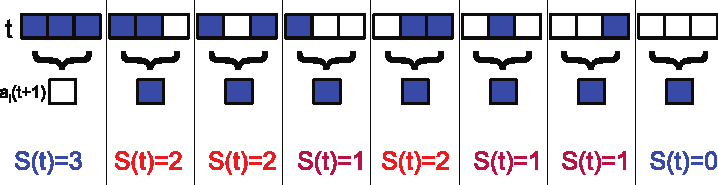
\includegraphics[width=0.8\textwidth]{img/task10}
	\caption{totalistic but illegal rule}
	\end{figure}
Disprove by contradicting example: The depicted rule is totalistic. But it is illegal, since it lacks a silent state, though it is symmetric.
\begin{solution}
\end{solution}

\begin{problem}[Assignment 11]
\end{problem}
\begin{solution}
\end{solution}

\begin{problem}[Assignment 12]
\end{problem}
\begin{solution}
${150}_D = {10010110}_B$
\begin{figure}[h!]
	\centering
	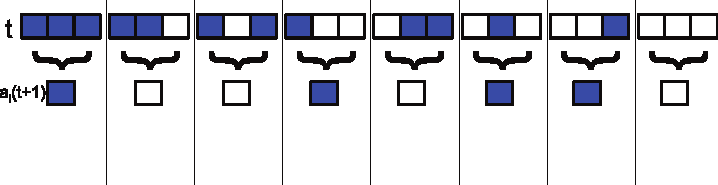
\includegraphics[width=0.8\textwidth]{img/task12}
	\caption{rule ${150}_D$}
\end{figure}

It follows: $S(t)=3 \Rightarrow 1, S(t)=2 \Rightarrow 0, S(t)=1 \Rightarrow 1, S(t)=0 \Rightarrow 0$.
Thus, the rule can be expressed by the formula: $\mod{(\sum_i a_i, 2)}$. The remainder of division by $2$ of the sum of the neighbourhood.

A cellular automaton for the rule is depicted in table \ref{tab:rule150}. The formula is implemented in the file \verb+task12.ods+. 

\begin{table}[h!]
	\centering
	\begin{tabular}{|c|c|c|c|c|c|c|c|c|c|c|c|}
	\hline
		0	&0	&1	&0	&0	&0	&1	&0	&1	&0	&0	&0\\
	\hline
		0	&1	&1	&1	&0	&1	&1	&0	&1	&1	&0	&0\\
	\hline
		0	&0	&1	&0	&0	&0	&0	&0	&0	&0	&1	&0\\
	\hline
		0	&1	&1	&1	&0	&0	&0	&0	&0	&1	&1	&0\\
	\hline
		0	&0	&1	&0	&1	&0	&0	&0	&1	&0	&0	&0\\
	\hline
		0	&1	&1	&0	&1	&1	&0	&1	&1	&1	&0	&0\\
	\hline
		0	&0	&0	&0	&0	&0	&0	&0	&1	&0	&1	&0\\
	\hline
		0	&0	&0	&0	&0	&0	&0	&1	&1	&0	&1	&0\\
	\hline
		0	&0	&0	&0	&0	&0	&1	&0	&0	&0	&1	&0\\
	\hline
		0	&0	&0	&0	&0	&1	&1	&1	&0	&1	&1	&0\\
	\hline
		0	&0	&0	&0	&1	&0	&1	&0	&0	&0	&0	&0\\
	\hline
		0	&0	&0	&1	&1	&0	&1	&1	&0	&0	&0	&0\\
	\hline
		0	&0	&1	&0	&0	&0	&0	&0	&1	&0	&0	&0\\
	\hline
		0	&1	&1	&1	&0	&0	&0	&1	&1	&1	&0	&0\\
	\hline
		0	&0	&1	&0	&1	&0	&1	&0	&1	&0	&1	&0\\
	\hline
		0	&1	&1	&0	&1	&0	&1	&0	&1	&0	&1	&0\\
	\hline
		0	&0	&0	&0	&1	&0	&1	&0	&1	&0	&1	&0\\
	\hline
		0	&0	&0	&1	&1	&0	&1	&0	&1	&0	&1	&0\\
	\hline
		0	&0	&1	&0	&0	&0	&1	&0	&1	&0	&1	&0\\
	\hline
		0	&1	&1	&1	&0	&1	&1	&0	&1	&0	&1	&0\\
	\hline 
	\end{tabular} 
\caption{$20$ steps of rule ${150}_D$, first row input is random input. Column $1$ and $12$ are fixed to $0$.}
\label{tab:rule150}
\end{table}
\end{solution}

\begin{problem}[Assignment 13]
\end{problem}
\begin{solution}
	\begin{enumerate}[a)]
		\item $Z = k^{k^{(2 \cdot r+1)}}$
		\item $Z_p = \frac{1}{2} \cdot k^{k^{(2 \cdot r+1)}}$
		\item $Z_t = k^{2^{(2 \cdot r+1)}-1}$, since in a $2 \cdot r + 1$ neighbourhood, their can be $2^{(2 \cdot r+1)}-1$ different sums (each cell having $k$ possible values).
		\item $Z_{pt} = \frac{1}{2} \cdot Z_t$
	\end{enumerate}
\end{solution}

\pagebreak

\begin{problem}[Assignment 14]
\end{problem}
	\begin{table}[h!]
		\centering
		\begin{tabular}{|c|c|c|c|c|c|c|c|c|c|}
		\hline  & $2^7$ & $2^6$ & $2^5$ & $2^4$ & $2^3$ & $2^2$ & $2^1$ & $2^0$ &  \\ 
		\hline  & 
\includegraphics[width=0.08\textwidth]{img/7B} & 
\includegraphics[width=0.08\textwidth]{img/6B} & 
\includegraphics[width=0.08\textwidth]{img/5B} & 
\includegraphics[width=0.08\textwidth]{img/4B} & 
\includegraphics[width=0.08\textwidth]{img/3B} & 
\includegraphics[width=0.08\textwidth]{img/2B} & 
\includegraphics[width=0.08\textwidth]{img/1B} & 
\includegraphics[width=0.08\textwidth]{img/0B} &  \\ 
		\hline
		\hline  & 
\includegraphics[width=0.03\textwidth]{img/0.pdf} & 
\includegraphics[width=0.03\textwidth]{img/0.pdf} & 
\includegraphics[width=0.03\textwidth]{img/0.pdf} & 
\includegraphics[width=0.03\textwidth]{img/0.pdf} & 
\includegraphics[width=0.03\textwidth]{img/0.pdf} & 
\includegraphics[width=0.03\textwidth]{img/0.pdf} & 
\includegraphics[width=0.03\textwidth]{img/0.pdf} & 
\includegraphics[width=0.03\textwidth]{img/0.pdf} &  \\ 
	      $0_D$ & 0 & 0 & 0 & 0 & 0 & 0 & 0 & 0 & l,t,p \\ 
		\hline  & 
\includegraphics[width=0.03\textwidth]{img/0.pdf} & 
\includegraphics[width=0.03\textwidth]{img/0.pdf} & 
\includegraphics[width=0.03\textwidth]{img/0.pdf} & 
\includegraphics[width=0.03\textwidth]{img/1.pdf} & 
\includegraphics[width=0.03\textwidth]{img/0.pdf} & 
\includegraphics[width=0.03\textwidth]{img/0.pdf} & 
\includegraphics[width=0.03\textwidth]{img/0.pdf} & 
\includegraphics[width=0.03\textwidth]{img/1.pdf} &  \\ 
		 $17_D$ & 0 & 0 & 0 & 1 & 0 & 0 & 0 & 1 & - \\  
		\hline  & 
\includegraphics[width=0.03\textwidth]{img/0.pdf} & 
\includegraphics[width=0.03\textwidth]{img/0.pdf} & 
\includegraphics[width=0.03\textwidth]{img/1.pdf} & 
\includegraphics[width=0.03\textwidth]{img/0.pdf} & 
\includegraphics[width=0.03\textwidth]{img/1.pdf} & 
\includegraphics[width=0.03\textwidth]{img/0.pdf} & 
\includegraphics[width=0.03\textwidth]{img/1.pdf} & 
\includegraphics[width=0.03\textwidth]{img/0.pdf} &  \\ 
		 $42_D$ & 0 & 0 & 1 & 0 & 1 & 0 & 1 & 0 & - \\  
		\hline  & 
\includegraphics[width=0.03\textwidth]{img/0.pdf} & 
\includegraphics[width=0.03\textwidth]{img/0.pdf} & 
\includegraphics[width=0.03\textwidth]{img/1.pdf} & 
\includegraphics[width=0.03\textwidth]{img/1.pdf} & 
\includegraphics[width=0.03\textwidth]{img/0.pdf} & 
\includegraphics[width=0.03\textwidth]{img/1.pdf} & 
\includegraphics[width=0.03\textwidth]{img/0.pdf} & 
\includegraphics[width=0.03\textwidth]{img/0.pdf} &  \\ 
		 $51_D$ & 0 & 0 & 1 & 1 & 0 & 1 & 0 & 0 & - \\  
		\hline  & 
\includegraphics[width=0.03\textwidth]{img/0.pdf} & 
\includegraphics[width=0.03\textwidth]{img/1.pdf} & 
\includegraphics[width=0.03\textwidth]{img/1.pdf} & 
\includegraphics[width=0.03\textwidth]{img/0.pdf} & 
\includegraphics[width=0.03\textwidth]{img/1.pdf} & 
\includegraphics[width=0.03\textwidth]{img/1.pdf} & 
\includegraphics[width=0.03\textwidth]{img/1.pdf} & 
\includegraphics[width=0.03\textwidth]{img/0.pdf} &  \\ 
		$110_D$ & 0 & 1 & 1 & 0 & 1 & 1 & 1 & 0 & - \\ 
		\hline  & \includegraphics[width=0.03\textwidth]{img/1.pdf} & \includegraphics[width=0.03\textwidth]{img/0.pdf} & \includegraphics[width=0.03\textwidth]{img/1.pdf} & \includegraphics[width=0.03\textwidth]{img/0.pdf} & \includegraphics[width=0.03\textwidth]{img/0.pdf} & \includegraphics[width=0.03\textwidth]{img/1.pdf} & \includegraphics[width=0.03\textwidth]{img/0.pdf} & \includegraphics[width=0.03\textwidth]{img/1.pdf} &  \\ 
		$165_D$ & 1 & 0 & 1 & 0 & 0 & 1 & 0 & 1 & s,p \\  
		\hline  & \includegraphics[width=0.03\textwidth]{img/1.pdf} & \includegraphics[width=0.03\textwidth]{img/1.pdf} & \includegraphics[width=0.03\textwidth]{img/0.pdf} & \includegraphics[width=0.03\textwidth]{img/0.pdf} & \includegraphics[width=0.03\textwidth]{img/1.pdf} & \includegraphics[width=0.03\textwidth]{img/1.pdf} & \includegraphics[width=0.03\textwidth]{img/0.pdf} & \includegraphics[width=0.03\textwidth]{img/0.pdf} &  \\ 
		$204_D$ & 1 & 1 & 0 & 0 & 1 & 1 & 0 & 0 & l \\ 
		\hline  & \includegraphics[width=0.03\textwidth]{img/1.pdf} & \includegraphics[width=0.03\textwidth]{img/1.pdf} & \includegraphics[width=0.03\textwidth]{img/1.pdf} & \includegraphics[width=0.03\textwidth]{img/1.pdf} & \includegraphics[width=0.03\textwidth]{img/0.pdf} & \includegraphics[width=0.03\textwidth]{img/0.pdf} & \includegraphics[width=0.03\textwidth]{img/1.pdf} & \includegraphics[width=0.03\textwidth]{img/1.pdf} &  \\ 
		$243_D$ & 1 & 1 & 1 & 1 & 0 & 0 & 1 & 1 & - \\  
		\hline 
		\end{tabular} 
	\caption{Wolfram numbers and rules: l=legal, t=totalistic, s=symmetric, p=peripheral}
	\end{table}
\begin{solution}
\end{solution}

\begin{problem}[Assignment 15]
\end{problem}
\begin{solution}
\end{solution}

\end{document}
